% Copyright (C) 2013 - Michael Baudin
%
% This file must be used under the terms of the 
% Creative Commons Attribution-ShareAlike 3.0 Unported License :
% http://creativecommons.org/licenses/by-sa/3.0/

\chapter{The Faure sequence}

\section{Principles}

    
      Let s be the number of dimensions.
      The Faure sequence uses the smallest prime number greater or equal than
      b.
      For example, if $s=6$, then the prime number b used by the Faure
      sequence is 7.
    

    
      Let k be an integer and let $a_i(k)$ be the coefficients of the
      base-b decomposition of k:
    

    
      $$
        k=\sum_{i=0}^{r-1} a_i(k) b^i.
      $$
    

    
      Let i be an integer in the set $\{1,2,...,s\}$.
      The i-th coordinate of the Faure sequence makes use of a r-by-r upper
      triangular matrix, called the generator matrix. 
	  For the Faure sequence, the generator matrix is based on the 
	  Pascal matrix defined as:
    

    
      $$
        C^{(i)}(m,n) = {n-1 \choose m-1} i^{n-m},
      $$
    

    
      where
    

    
      $$
        {n-1 \choose m-1} = \frac{m!}{n!(m-n)!}
      $$
    

    
      for $$n\geq m$$ and zero otherwise.
    

    
      By convention $C^{(0)}$ is identity matrix.
    

    
      Consider the column vector $a(k)$ defined by ordering the
      digits from the least significant to the most significant:
    

    
      $$
        a(k)=(a_0(k),a_1(k),...,a_{r-1}(k))^T.
      $$
    

    
      We introduce the column vector $y(k)$ defined by the matrix-vector product:
    

    
      $$
        y^{(i)}(k) = C^{(i-1)} a(k) \pmod b
      $$
    

    
      The i-th component of the Faure sequence is:
    

    
      $$
        x^{(i)}_k = \sum_{i=0}^{r-1} y^{(i)}(k)b^{-i-1}.
      $$
    

%%%%%%%%%%%%%%%%%%%%%%%%%%%%%%%%%%%%%%%%%%%%%%%%%%%%%%%%%%%%%%%%%%
\section{Properties}

    
      The matrices $C^{(i)}$ are so that  
      $$
        C^{(i)} a(k) \pmod b
      $$
      is a permutation of the vector $a(k)$ for the set of points
      $k=jb^r,...,(j+1)b^r-1$, for any $j=0,1,...,b-1$.
      Hence, for this set of points, each component $x^{(i)}_k$ is a
      permutation of the Van Der Corput sequence $\psi_b(k)$.
    
      The first component of the Faure sequence is the Van Der Corput sequence
      in base $b$.
      Other components of the Faure sequence are permutations of sub-sequences
      of the Van Der Corput sequence in base $b$.
    

    
      Faure sequences are (0,s)-sequences in base $b$.
      Therefore, Faure sequences have the lowest possible value
      of the quality parameter $t$ in base $b$.
      On the other hand, the base increases with the dimension $s$,
      although the base for the Faure sequence increases much
      slower than the largest base of the Halton sequence.
    
%%%%%%%%%%%%%%%%%%%%%%%%%%%%%%%%%%%%%%%%%%%%%%%%%%%%%%%%%%%%%%%%%%
\section{Examples}

    
      The following function computes the Faure matrix,
      given the number of digits $r$ and the dimension index $i$.
    

\lstset{language=scilabscript}
\begin{lstlisting}
function c = faurematrix ( r , i )
    c = zeros(r,r)
    for m = 1:r
        b=specfun_nchoosek ((m:r)-1 , m-1)
        c(m,m:r) = i.^((m:r)-m) .* b
    end
endfunction
\end{lstlisting}

    
      For r=1, the Faure matrix is equal to one.
      The following script prints the Faure matrices for increasing
      values of r and i.
    

\lstset{language=scilabscript}
\begin{lstlisting}
for r=2:3
    for i=1:3
        c = faurematrix ( r , i );
        mprintf("r=%d, C(%d)\n",r,i)
        disp(c)
    end
end
\end{lstlisting}

    
      The previous script produces the following output.
    

\lstset{language=scilabscript}
\begin{lstlisting}
r=2, C(1)
    1.    1.  
    0.    1.  
r=2, C(2)
    1.    2.  
    0.    1.  
r=2, C(3)
    1.    3.  
    0.    1.  
r=3, C(1)
    1.    1.    1.  
    0.    1.    2.  
    0.    0.    1.  
r=3, C(2)
    1.    2.    4.  
    0.    1.    4.  
    0.    0.    1.  
r=3, C(3)
    1.    3.    9.  
    0.    1.    6.  
    0.    0.    1.  
\end{lstlisting}

    
      The following script produces the first 10 points
      of the Faure sequence in s=3 dimensions.
      For this value of s, the Faure sequence uses the base b=3.
      We use the \scifun{number\_tobary} function in order
      to decompose the integer k into base b.
      The "bigendian" option reverses the order of the digits,
      so that the most significant digit comes last.
      Then we compute the matrix-vector product \scivar{C*a}
      and compute the remainder modulo b.
      Finally, we evaluate the point by using powers of the
      inverse of b.
    

\lstset{language=scilabscript}
\begin{lstlisting}
b=3;
s=3;
for k=1:10
    a=number_tobary(k,b,"bigendian");
    r=size(a,"*");
    bpow=b.^(1:r)';
    for i=1:s
        C=faurematrix ( r , i-1 );
        y=modulo(C*a,b);
        x(k,i)=sum(y./bpow);
    end
end
disp(x)
\end{lstlisting}

    
      The previous script produces the following output.
    

\lstset{language=scilabscript}
\begin{lstlisting}
-->disp(x)
    0.3333333    0.3333333    0.3333333  
    0.6666667    0.6666667    0.6666667  
    0.1111111    0.4444444    0.7777778  
    0.4444444    0.7777778    0.1111111  
    0.7777778    0.1111111    0.4444444  
    0.2222222    0.8888889    0.5555556  
    0.5555556    0.2222222    0.8888889  
    0.8888889    0.5555556    0.2222222  
    0.0370370    0.5925926    0.4814815  
    0.3703704    0.9259259    0.8148148  
\end{lstlisting}

    
      We can compare with the second component of the
      Halton sequence in s=2 dimensions, which uses the
      prime number b=3 as the base.
    

\lstset{language=scilabscript}
\begin{lstlisting}
u=lowdisc_ldgen(10,2,"halton");
u(:,2)
\end{lstlisting}

    
      The previous script produces the following output.
    

\lstset{language=scilabscript}
\begin{lstlisting}
-->u(:,2)
 ans  =
    0.3333333  
    0.6666667  
    0.1111111  
    0.4444444  
    0.7777778  
    0.2222222  
    0.5555556  
    0.8888889  
    0.0370370  
    0.3703704  
\end{lstlisting}

%%%%%%%%%%%%%%%%%%%%%%%%%%%%%%%%%%%%%%%%%%%%%%%%%%%%%%%%%%%%%%%%%%
\section{Properties of 1D projections}

    
      The following script computes the elements of the first 27 
	  points of the Faure sequence in 3 dimensions. 
	  We plot the first component at the top, the second component 
	  in the middle and the third component at the bottom. 
	  We see that all the points in each coordinate are at the 
	  same positions, but come in a different order. 
	  This point set is made, indeed, of permuted point sets 
	  from the Van Der Corput sequence in base b=3.
    

\lstset{language=scilabscript}
\begin{lstlisting}
s=3;
b=3;
scf();
lds = lowdisc_new("faure");
lds = lowdisc_configure(lds,"-dimension",s);
k=1;
imax=3;
for i=1:imax
    npoints=(b-1)*b^(i-1);
    [lds,u]=lowdisc_next(lds,npoints);
    for j=1:s
        subplot(s,1,j)
        plot(u(:,j)',i,"bo")
        xstring(u(:,j)',i,string(k:k+npoints-1))
    end
    k=k+npoints;
end
lds = lowdisc_destroy (lds);
for j=1:s
    subplot(s,1,j)
    a = gca();
    a.data_bounds=[
    0 0
    1 imax+1
    ];
    xtitle("Faure Sequence","X"+string(j),"Block Index")
end
\end{lstlisting}
    
	
The previous script produces the figure \ref{fig-faure-s3-n27}.

\begin{figure}[htbp]
\begin{center}
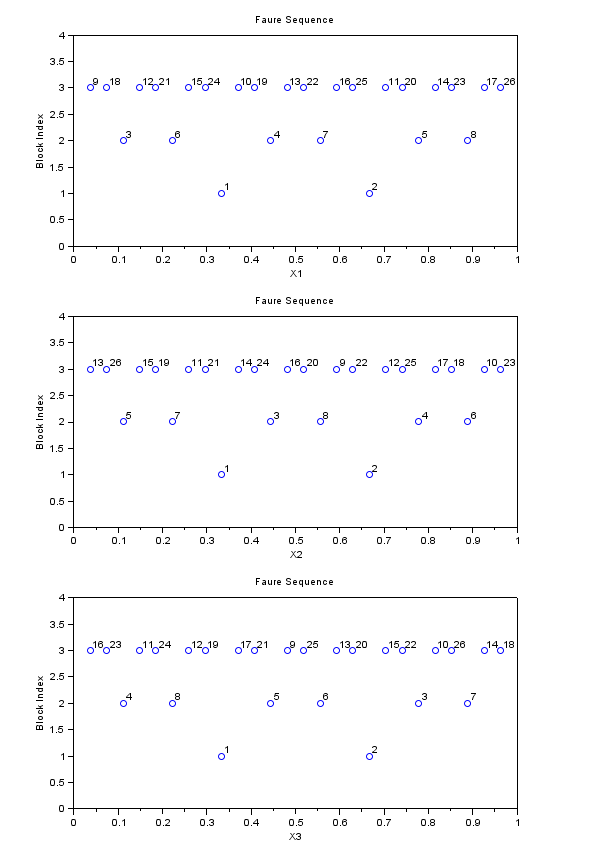
\includegraphics[width=15cm]{figures/faure-s3-n27.png}
\end{center}
\caption{The Faure sequence - Projections of n=27 points in s=3 dimensions.}
\label{fig-faure-s3-n27}
\end{figure}

    
      We can also look at the distribution of sub-sequences 
	  of the Faure point set in s=3 dimensions. 
	  In the following script, we consider a set of $3^4=81$ points, 
	  organized in 3 consecutive blocks of $3^3=27$ points. 
	  We plot the first component at the top, the second component 
	  in the middle and the third component at the bottom. 
	  The goal of this experiment is to visualize the point sets 
	  with indices $ib^r,...,(i+1)b^r-1$, for $i=0,1,...,b-1$ 
	  with r=2. 
	  We can see these particular sub-sequences of consecutive 27 points are 
	  evenly filling the one dimensionnal interval $[0,1]$, 
	  so that the sub-sequences are translated by $1/27$ each 
	  time a new block $i$ is considered. 
    

\lstset{language=scilabscript}
\begin{lstlisting}
b=3;
s=3;
u=lowdisc_ldgen(3^3,3,"faure");
u=[zeros(1,s);u];
scf();
npoints=b^3;
for i=0:b-1
    for j=1:s
        subplot(s,1,j)
        indices=i*b^2+1:(i+1)*b^2
        plot(u(indices,j)',i,"bo")
        xstring(u(indices,j)',i,string(indices))
    end
end
for j=1:s
    subplot(s,1,j)
    a = gca();
    a.data_bounds=[
    0 -1
    1 b
    ];
    xtitle("Faure Sequence","X"+string(j),"Block Index")
end
\end{lstlisting}

The previous script produces the figure \ref{fig-faure-s3-n27-B}.
    
\begin{figure}[htbp]
\begin{center}
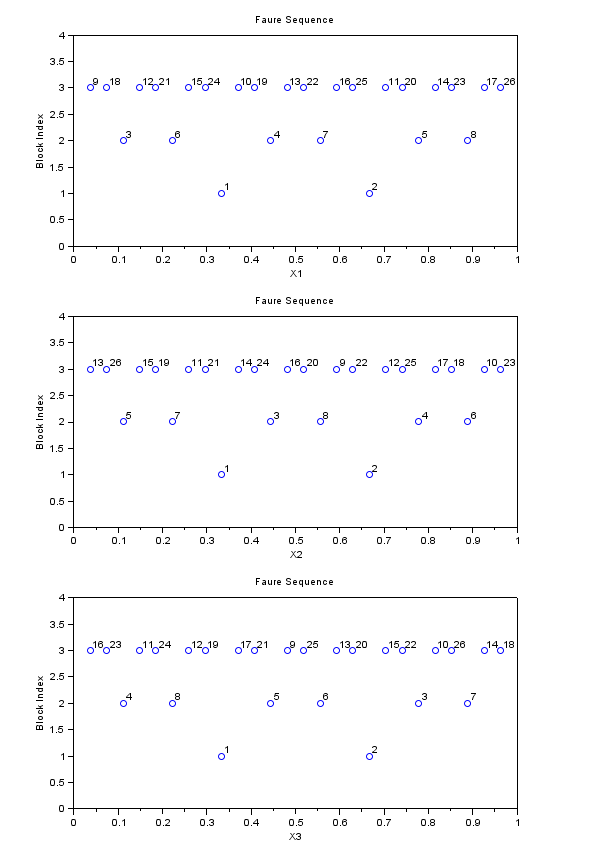
\includegraphics[width=15cm]{figures/faure-s3-n27.png}
\end{center}
\caption{The Faure sequence - Projections of n=27 points in s=3 dimensions.}
\label{fig-faure-s3-n27-B}
\end{figure}
    
%%%%%%%%%%%%%%%%%%%%%%%%%%%%%%%%%%%%%%%%%%%%%%%%%%%%%%%%%%%%%%%%%%
\section{Value of the prime base}

    
      One potential advantage of the Faure sequence over the Halton 
	  sequence is that the prime base is much smaller than the 
	  largest prime used in the Halton sequence. 
	  This is the prime number used by the s-th component of the 
	  sequence. 
	  This is because, in s dimensions, the Halton sequence uses 
	  the prime numbers $p(1),p(2),...,p(s)$, while the Faure 
	  sequence only uses the smallest prime larger or equal to n.
    

    
      The following script compares the base used by the Faure 
	  sequence for $s=1,2,...,100$ and compare it to the largest 
	  base used by the Halton sequence. 
    

\lstset{language=scilabscript}
\begin{lstlisting}
p=number_primes100();
scf();
plot(1:100,p,"r-")
b=[];
for n=1:100
    k=find(p>n,1);
    b(n)=p(k);
end
plot(1:100,b,"b-")
legend(["Halton Largest Base" "Faure Base"]);
xtitle("","Number of Dimensions","Prime Base")
\end{lstlisting}
	
    
      We can see in the figure \ref{fig-faure-base} 
	  that the Halton sequence can make use of 
	  much larger bases, which potentially leads to much 
	  larger number cycles. 
    

\begin{figure}[htbp]
\begin{center}
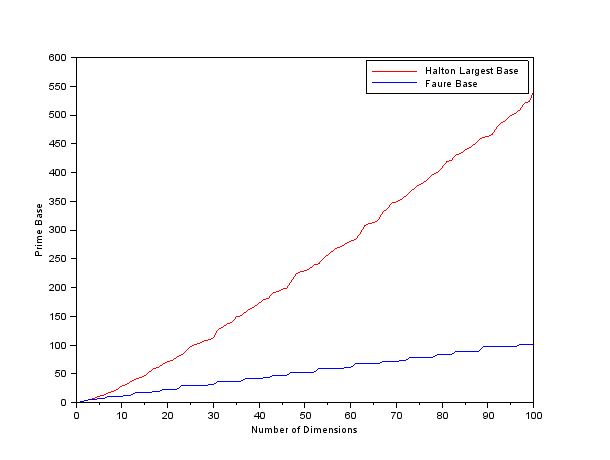
\includegraphics[width=15cm]{figures/faure-base.png}
\end{center}
\caption{The base used in the Faure sequence compared with the largest base used in the Halton sequence.}
\label{fig-faure-base}
\end{figure}
    
      However, the lowest components of the Halton sequence 
	  may make use of potentially much smaller bases than the 
	  equivalent Faure sequence. 
	  Indeed, if the user of a Halton sequence orders the 
	  variables so that the most important variables come 
	  first, then the Halton sequence can potentially lead 
	  to better results. 
	  On the other hand, the Faure sequence does not favor 
	  any component, which may be safer in the general situation where 
	  we do not know in advance which variable may be important. 
    

%%%%%%%%%%%%%%%%%%%%%%%%%%%%%%%%%%%%%%%%%%%%%%%%%%%%%%%%%%%

\section{Notes and references}

Most of the theoretical content of this chapter is based on Glasserman's \cite{Glasserman2003}.
